\documentclass[fontsize=12pt,openright,twoside,paper=a4,BCOR=1cm]{scrbook}
\DeclareOldFontCommand{\bf}{\normalfont\bfseries}{\mathbf}

\newcommand{\authornamefirst}{Michael}
\newcommand{\authornamemiddle}{J.}
\newcommand{\authornamelast}{Ehrlinger}
\newcommand{\worktitle}{Improving Quality of Service for Electric Vehicle Charging in the Low Voltage Grid using Slotted ALOHA Protocol}
\newcommand{\thesistype}{Bachelor Thesis}
\newcommand{\thesisdate}{xx/03/2020}
\newcommand{\thesisprof}{Prof. Dr.-Ing. Hermann de Meer}
\newcommand{\thesissecondprof}{??}
\newcommand{\supervisor}{Dominik Danner,~M.~Sc.}
\newcommand{\chair}{Chair of Computer Networks \& Communications}

\newcommand{\contactprofone}{
\thesisprof \\
\chair \\
Universit\"at Passau \\
E-Mail:~{\small \url{demeer@fim.uni-passau.de}}  \\
Web:~{\small
\url{http://www.net.fim.uni-passau.de/}}\\}

\newcommand{\contactproftwo}{
\thesissecondprof \\
Chair of XYZ \\
Universit\"at Passau \\
E-Mail:~{\small \url{xxx@fim.uni-passau.de}}  \\
Web:~{\small
\url{http://www.xxx.fim.uni-passau.de/}}\\}


\newcommand{\contactsupervisor}{
\supervisor \\
\chair \\
Universit\"at Passau \\
E-Mail:~{\small \url{xxx@fim.uni-passau.de}}  \\
Web:~{\small
\url{http://www.xxx.fim.uni-passau.de/}}\\}



%%%%%%%%%%%%%%%%%%%%%%%%%%%%%%%%%%%%%%%%%%%%%%%%%%%%%%%%%%%%

% PACKAGES:





% Use English :

% Use list of tabels, etc. in table of contents:
\usepackage{tocbibind}
% German paragraph skip
\usepackage{parskip}
\usepackage[utf8]{inputenc}
% Index-generation
\usepackage{makeidx}
% Einbinden von URLs:
\usepackage{url}
% Include .eps-files (needed also for the CNACC-logo):
%\usepackage{epsf}
% Special \LaTex symbols (e.g. \BibTeX):
\usepackage{doc}
% Include Graphic-files:
%\usepackage{graphics}
% Include Graphic-files:
\usepackage{graphicx}
\usepackage{acronym}
% Include doc++ generated tex-files:
%\usepackage{docxx}
% Include PDF links

%mathstuff
\usepackage[cmex10]{amsmath}
\usepackage{amsfonts}
\usepackage{amssymb}
\usepackage{listings}
\usepackage{booktabs}

%hyperref for nice PDF output
\usepackage[pdftex, bookmarks=true]{hyperref}

%%%%%%%%%%%%%%%%%%%%%%%%%%%%%%%%%%%%%%%%%%%%%%%%%%%%%%%%%%%%

% OTHER SETTINGS:

% Pagestyle:
\pagestyle{headings}

% Avoid 'overhang':
\sloppy

% Choose language
\newcommand{\setlang}[1]{\selectlanguage{#1}\nonfrenchspacing}

\usepackage[USenglish, german]{babel}


%%%%% 	CHANGE THE LANGUAGE HERE! %%%%%%%%
%\setlang{USenglish}
\setlang{german}

%%%%%%%%%%%%%%%%%%%%%%%%%%%%%%%%%%%%%%%%%%%%%%%%%%%%%%%%%%%%

% TITLE:

\begin{document}

\thispagestyle{empty}
\newpage

\vspace{1cm}

\begin{center}
\begin{tabular}{lr}

\includegraphics[width=6.5cm]{img/logouni.pdf}
&

\includegraphics[width=6.5cm]{img/logochair.pdf}
\end{tabular}

\vspace{3cm}
\Large University of Passau
\\
\Large Faculty of Computer Science and Mathematics
\\
\vspace{0.3cm}
\Large {\bf \chair }
\\
\Large \thesisprof

\end{center}


\vspace{4.5cm}

\begin{center}
        {\bf\Huge \thesistype} % Master Thesis, Programming Project
\end{center}

\begin{center}
        \settowidth{\baselineskip}{0.4cm}
        {\LARGE \worktitle}
        \\
        {\Large
        \authornamefirst~\authornamemiddle~\authornamelast
        }
\end{center}

\vfill {% \settowidth{\baselineskip}{0.2cm}

\vfill


{\large
\begin{tabular}[l]{llll}

Date:       & \thesisdate %%(\LaTeX{}$2_\epsilon$ run \today)
\smallskip \\
Supervisors:   & \thesisprof \\
&\thesissecondprof \\
	& \supervisor \\
\end{tabular}}
} \cleardoublepage
%%%%%%%%%%%%%%%%%%%%%%%%%%%%%%%%%%%%%%%%%%%%%%%%%%%%%%%%%%%%



% MAIN PART:

% Erklärung
%
\thispagestyle{empty}

\begin{center}
\huge{\textbf{Erklärung zur \thesistype}}
\end{center}

\vspace{4cm}
Name, Vorname des\\Studierenden: \hspace{4cm} \authornamelast,~\authornamefirst~\authornamemiddle
\vspace{2cm}
\\Universität Passau,\\
Fakultät für Informatik und Mathematik
\vspace{3cm}
\begin{center}
Hiermit erkläre ich, dass ich die Arbeit selbstständig verfasst, noch nicht anderweitig
für Prüfungszwecke vorgelegt, keine anderen als die angegebenen Quellen oder Hilfsmittel
benutzt, sowie wörtliche und sinngemäße Zitate auch als solche gekennzeichnet habe. Die Arbeit, 
oder Teile davon, wurden weder von mir noch von einer anderen Person an der Universität Passau 
oder an einer andern Hochschule zur Erlangung eins akademischen Titels bereits eingereicht.

\end{center}
\vspace{4.5cm}
.........................\hfill....................................................\\
~~~(Datum)\hfill(Unterschrift des Studierenden)

\cleardoublepage
~
\vfill


{\bf{Supervisor Contacts:}} \smallskip \\
\contactprofone\\
\contactsupervisor\\

\cleardoublepage
%\thispagestyle{plain}

\section*{Abstract}
Das Problem eines Spannungsabfalls in einem Niederspannungsnetz, nachdem die angeschlossenen Teilnehmer eine zu hohe Last gezogen hat, motiviert eine Untersuchung. Das Stromnetz-Szenario mit zu vielen Benutzer, die das Stromnetz zum Beispiel zum Aufladen von Elektroautos nutzen, können als ein, aus der Netzwerktechnik bekanntes Problem, des multiple access angesehen werden. Ein Beispiel für einen multiple access Protokoll ist das ALOHA-Protokoll. Das Aloha-Protokoll wurde erfunden in 1970 für die Koordinierung und Vermittlung des Zugangs zu einem gemeinsamen Kommunikationsnetz, dies bedeutet, dass es in die Klasse der Mehrfachzugriffsprotokolle fällt. Das Aloha Netzwerkprotokoll arbeitet dezentral am jeweiligen Teilnehmer ohne zentrale Schnittstelle.Es gibt zwei Formen des ALOHA-Protokolls, pure und slotted ALOHA. Durch die Verwendung dieses Protokolls soll die Handhabung von hohen Lasten verbessert werden, welche auf einem Niederspannungsnetz beim Aufladen mehrerer Elektrofahrzeuge wirken. Das ALOHA Protokoll arbeitet mit Wartezeiten, nachdem eine Kollision aufgetreten ist. Es wurden zwei Varianten zur Bestimmung einer solchen Wartezeit erarbeitet, die erste Variante  verwendet lediglich die aktuelle Anzahl von ladebereiten Teilnehmern, die zweite Variante verwendet zusätzlich fahrzeugspezifische Parameter, wie Abfahrtszeit und Ladestand der Batterie. Neben einem Spannungskontroller wurde auch ein Transformatorkontroller entwickelt, welcher auf die vom Transformatorbezogene Leistung reagiert.\\
Die Bewertung der zuvor genannten Methoden erfolgt mithilfe des co-Simulationsframeworks Mosaiks, das einen Stromflusssimulator (PyPower) und unsere Implementierung des ALOHA-Algorithmus. Dieser Co-Simulator benötigt für einen funktionierenden Betrieb ein vordefiniertes Netz, hier wurde das IEEE906, ein repräsentatives europäischen Niederspannungsnetz, verwendet. Die nach der Simulation erhaltenen Ergebnisse zeigen, dass im vorliegenden Szenario die Verwendung beider ALOHA Varianten Vorteile bezüglich dem herkömmlichen Spannungsregelung bieten. Nicht nur wird die Spannungsqualität verbessert und der Leistungsbezug harmonisiert, sondern auch die Fairness zwischen den Teilnehmer wird gehalten und teils auch verbessert. Die Verbesserungen am Spannungscontroller ermöglichen bereits eine Verbesserung der Spannungswerte, wenn allerdings der Transformatorkontroller ebenfalls verwendet wird, wird auch die Lastverteilung auf das Niederspannungsnetz verbessert. Beide Verbesserungen an sich sind für sich bereits erstrebenswert, das beste Ergebnis zeigte sich aber als beider Controller gemeinsam verwendet wurden. Es zeigt sich auch, dass die Verwendung von Teilnehmerzahl und Fahrzeugparametern zur Bestimmung der Wartezeiten dazu geeignet ist längere Wartezeiten zu bestimmen und somit die Ladevorgänge der einzelnen Teilnehmer besser zu verteilen.

%\tableofcontents


%\chapter{Einleitung}

Die Zahl der Elektrofahrzeuge in Deutschland nimmt immer weiter zu. Während es 2018 noch 98280 Fahrzeuge (Plug-In Hybride und Elektrofahrzeuge) waren es bereits 2019 66997 Plug-In Fahrzeuge und 83175 Elektrofahrzeuge, also 51892 mehr Fahrzeuge (Statsita1). Sowohl Plug-In Hybride als auch Elektrofahrzeuge können über ein Ladegerät mit elektrischem Strom versorgt werden. Laut einer Statistik über die bevorzugten Ladeorte für Elektrofahrzeuge ist das Zuhause des Fahrzeughalters der beliebteste Ort zum Aufladen des Fahrzeuges (Statista2). Haushalte in Deutschland sind prinzipiell mit dem Niederspannungsnetz verbunden. \\
Das deutsche Niederspannungsnetz arbeitet gemäß DIN EN 50160 mit Wechselstrom bei 230 Volt Normspannung und einer Frequenz von 50 Hz. Wenn nun aber eine große Last auf ein Niederspannungsnetz wirkt, sinkt die Spannung im Netz ab. Sinkt die Spannung zu weit ab, wird die Leistung der betroffenen Geräte zurückgefahren, dies kann bedeuten, dass Geräte nur noch wenig bis keine Leistung mehr liefern können. Im Falle der bereits erwähnten Ladegeräte würde dieses Zurückfahren der Leistung bedeuten, dass die Länge des Ladevorgangs vergrößert wird, wodurch das Fahrzeug erst später wieder zur vollen Verfügung steht. Nun stellen aber gerade die zunehmenden Ladevorgänge der wachsenden Zahl von Elektrofahrzeugen in Deutschland die betroffenen Niederspannungsnetze vor eine große Herausforderung. Die Herausforderung liegt in der Leistung, die jeder einzelne Ladevorgang benötigt. Die Summe dieser Vorgänge, welche auf das Niederspannungsnetz wirken, können nämlich ein Absinken der Spannung zur Folge haben. Dieses Absinken der Spannung tritt vor allem dann auf, wenn ohnehin schon viele Verbraucher Leistung beziehen. Bei einem hohen Leistungsbezug ohne dem laden vom Elektrofahrzeugen, sorgt der zusätzliche bedarf dafür zu einem noch weiterem Absinken der Spannung. Diese Absinken führt zu einer schlechteren Erfahrung bei der Verwendung des Niederspannungsnetzes, nicht nur beim laden von Elektrofahrzeugen, sondern auch bei der herkömmlichen Verwendung. Um dem Absinken bei steigender Last entgegen zu wirken, sehen sich Netzbetreiber, wie etwa E.ON, gezwungen in ihre Netze zu investieren, um den zukünftigen Belastungen besser standzuhalten. \\
Der Netzbetreiber E.ON hat in einer Pressemitteilung bekanntgegeben in den nächsten 25 Jahren, also bis zum Jahre 2045, rund 2,5 Milliarden Euro in seine Netze investieren zu wollen. Im Netzgebiet von E.ON gibt es laut ihrer Aussage aktuell etwa 6,5 Millionen konventionelle Pkw, im Jahre 2045 will E.ON in der Lage sein all diese Pkw mit den dann ausgebauten Netzen mit elektrischer Energie zu versorgen. Verteilt man die 2,5 Milliarden Euro auf die 6,5 Millionen Fahrzeuge, ergeben sich pro Fahrzeug etwa 400 Euro. Der Netzbetreiber schätzt allerdings, dass sich diese Zahl noch senken lässt, etwa durch den Einsatz intelligenter Steuerungen. \\
Ein Ansatz zu einer solchen intelligenten Steuerung wird in dieser Arbeit formuliert. Es wird untersucht, ob die Adaption des Aloha Protokolls auf das Niederspannungsnetz dazu beitragen kann, das Laden von Elektroautos und die damit einhergehende Last auf Stromnetz besser zu verteilen. Ein besonderes Augenmerk liegt auf der Verteilung der Leistung zwischen den einzelnen Teilnehmern um eine möglichst faire Verteilung der jeweils zur Verfügung stehenden Last zu erreichen. Um dies beurteilen zu können werden verschieden Ansätze zuerst vorgestellt und dann miteinander verglichen. Es werden verschieden Ansätze, welche mit dem Prinzip des Aloha Protokolls arbeiten vorgestellt. Ein weiterer dargestellter Ansatz fungiert als Kontrollgruppe, da dabei eine herkömmliche Anschlussregel, gemäß einer VDE-Norm verwendet wird.
\chapter{Background}
\label{chap:background}
\section{Setting}
\label{cap:background_sec:setting}
Hallo dies ist ein kurzer Test
\section{Reiner VDE-Controller}

% Main part can have multiple chaper-files, e.g.:
%\chapter{Verwendete Methodiken}
Nach der Einführung zu den verschieden Themenbereichen, nun zu den eigentlichen Methodiken, welche entweder schon vorhanden sind, oder im Zuge dieser Arbeit erarbeitet wurden.
\section{Ladeservice und Ladeprozess}
Ein Ladeservice startet, wenn ein Elektrofahrzeug mit einem passenden Ladegerät verbunden wird und endet, wenn eben diese Verbindung wieder getrennt wird. Während dieser Zeit soll sich der Ladezustand des Fahrzeuges entweder auf 100\% erhöhen, oder wenn dies, aufgrund von zeitlichen oder technischen Limitierungen nicht möglich ist, möglichst nah an 100\% annähern. Die Qualität des Ladeservices hängt vom Ladezustand des Elektrofahrzeuges bei Beendigung des Ladeservices ab. Je geringer der Abstand zu einem Ladezustand von 100\% desto höher ist die Qualität eines Ladeservice. Die Erhöhung des Ladezustands geschieht durch Ladevorgänge. Ein Ladeservice kann mehrere Ladevorgänge beinhalten. Die bloße Anzahl von Ladevorgängen in einem Ladeservice mindert potenziell nicht die Qualität des Services. Ein Ladevorgang erhöht den Ladezustand der Batterie durch Verwendung von elektrischer Energie, welche aus dem Netz bezogen wird. Ein Ladevorgang ist zeitlich unbeschränkt und endet wegen technischen Limitierungen oder wenn der Ladeservice, welcher den Ladevorgang enthält, endet. Technische Limitierung welche das Ende eines Ladeprozesses verursachen sind das nicht einhalten von Schwellenwerten in Hinsicht auf Spannung, Ladezustand des Fahrzeuges und Belastungen im Stromnetz. Im Ladevorgang selbst werden Geräte verwendet, welche elektrischen Strom benötigen, wenn dieser Strom nicht bei ausreichender Spannung vorliegt, muss der Ladevorgang abgebrochen werden. Ein Elektrofahrzeug kann keinen Ladezustand von mehr als 100\% aufweisen, werden bei einem Ladevorgang 100\% Ladezustand erreicht werden, endet der Ladevorgang. Bei einer zu hohen Belastung am Stromnetz wird im Sinne der Materialschonung der Ladevorgang beendet. Die Beendigung eines Ladevorgangs ist nicht gleichzusetzen mit dem Ende des Ladeservice an sich. 
\begin{figure}[tb]
	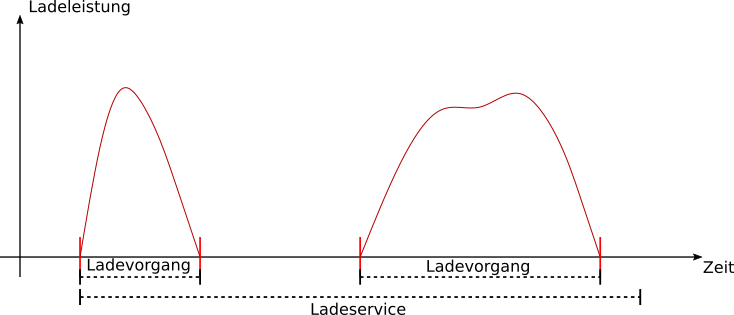
\includegraphics[width=\linewidth]{img/Ladeservice.png}
	\caption{Verlauf eines Ladeservices}
	\label{Abb_Ladeservice}
\end{figure}

In der Abbildung \ref{Abb_Ladeservice} wird die Aktivität innerhalb eines Ladeservices aufgezeigt. Der dargestellte Ladeservice enthält zwei Ladevorgänge. Die Länge beider Ladevorgänge zusammen ist kürzer als die Länge des Ladeservices.
\section{Datengrundlage}
\label{cap:background_sec:setting}
Während eines Ladeservices kann für die Beurteilung der aktuellen Situation auf verschiedene Daten zugegriffen werden. Es ist die Ankunftszeit, also der Beginn des Ladeservices, bekannt, ebenso wie die Abfahrtszeit, welche das Ende des Ladeservices markiert. Neben der Anfangs- und Endzeit, ist auch der aktuelle Zeitpunkt bekannt. Die aktuelle Zeit erhöht sich periodisch um immer den selben Wert und kann so in diskrete Zeiteinheiten eingeteilt werden. Des weiteren ist in jedem Zeitpunkt des Ladeservices der Ladezustand des Fahrzeuges, die aktuelle Spannung am Anschlusspunkt und die maximale nutzbare Stromstärke des Fahrzeuges des jeweiligen Teilnehmers bekannt. Über ein Broadcastsystem wird innerhalb eines Anschlussbereiches von jedem Teilnehmer, welcher aktuell einen Ladeservice durchführt, die Information das ein solcher Prozess stattfindet verteilt. Über das selbe Broadcastsystem wird von den Transformatoren des Anschlussbereiches die aktuelle Menge an Scheinleistung, welche in den Anschlussbereich abgegeben wird verteilt. Durch Sammlung der Meldungen von Fahrzeugen, welche gerade einen Ladeservice durchführen, lässt sich die Anzahl der aktuell stattfindenden Ladeservices im Anschlussbereich ermitteln. Der Anschlussbereich in dem diese Daten verbreitet werden umfasst jeweils ein einzelnes Niederspannungsnetz.  Es wird in dieser Arbeit im folgenden davon ausgegangen, das das verwendete Broadcastsystem keinen nennenswerten Delay aufweist und eine hohe Verfügbarkeit hat. Somit wird davon ausgegangen das die Daten immer übertragen werden und so immer verwendet werden können.

\section{Spannungsregler nach VDE 4100}
\label{capBody:VDE}
Die erste Methodik dient als Grundlinie für den Vergleich der später folgenden Methodiken. Diese Methodik stellt die aktuell im Stromnetz vorliegende Situation dar. Sie verwendet die technische Anschlussregel Niederspannung (VDE-AR-N 4100), diese stellt neue Anforderungen an die Ladegeräte von Elektrofahrzeugen. Sie wurde ebenfalls entwickelt, um eine größere Anzahl von Ladegeräten am Netz nutzbar zu machen \cite{kutter2020}. Bei der verwendeten Form der Anschlussregel, handelt es sich um einen Spannungsregulator, welcher anhand der Spannung angibt, wie viel der aktuell möglichen Leistung abgerufen wird. Bei einem gemessenen Wert der Spannung von mehr als 93\% der Normspannung, kann die Leistung wie gefordert abgerufen werden. Ab einer Spannung von weniger als 88\% der Normspannung kann keine Leistung mehr angerufen werden. In dem Bereich von 93\% bis 88\% der Normspannung wird die abrufbare Leistung linear reduziert, von voller hin zu keiner abrufbaren Leistung.

\begin{figure}[htb]
	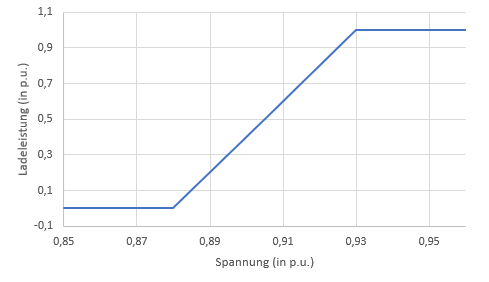
\includegraphics[width=\linewidth]{img/VDE3.png}
	\caption{Spannungs zu Leistungsverhältnis nach VDE-AR-N 4100}
	\label{Abb_VDEController}
\end{figure}

Der Graph in Abbildung \ref{Abb_VDEController} zeigt die mögliche Ladeleistung bei dem prozentualen Anteil der Normspannung. Auf der Y-Achse ist die mögliche Ladeleistung angetragen, wobei eins für die höchstmögliche Leistung steht und null dafür, dass für keine Leistung abrufbar ist. An der X-Achse werden die aktuell anliegenden Prozent der Normspannung angetragen. An dem Graphen ist ersichtlich, dass bei mehr als 93\% der Normspannung die ganze Ladeleistung zur Verfügung steht. Es ist weiterhin erkennbar, wie sich die mögliche Ladeleistung im Bereich von 93\% bis 88\% der Normspannung verhält. Ebenso ist erkennbar, wie das keine Ladeleistung bei einem Wert von weniger als 88\% der Normspannung mehr möglich ist. \\
Die Ladeleistung P\textsubscript{L} wird berechnet mithilfe der aktuellen Spannung U\textsubscript{A} und der aktuell maximal nutzbaren Stromstärke I\textsubscript{F} des Fahrzeuges durch die Formel
\begin{align}
	P\textsubscript{L} = U\textsubscript{A} \cdot I\textsubscript{F} \label{Main_formula1}
\end{align}
Bei der Formel \ref{Main_formula1} wird von einer Spannung von über 93\% der Normspannung ausgegangen, da die berechnete Ladeleistung nicht verändert wird. Im Bereich von unter 93\% der Normspannung ist eine solche Änderung aber nötig. Der Faktor F, mit dem der verbliebene Anteil der möglichen Ladeleistung berechnet wird, wird wie folgt bestimmt \\
\begin{center}
	$ F = \begin{cases}
	1 &  \text{$>$ 93\% Normspannung} \\
	0 &  \text{$<$ 88\% Normspannung} \\
	20 \cdot \frac{U\textsubscript{A}}{U\textsubscript{N}} - 17.6 & \text{$>$ 88\%, $<$ 93\% Normspannung}
	\end{cases}
	$
\end{center}
Der Wertebereich der Formel ist bei Null bzw. Eins abgeschlossen. Bei zu niedrigen Spannungswerten, weniger als 88\% der Normspannung, wird der Faktor ohne Berechnung der Formel mit null angegeben. Ergebnisse größer als eins werden auf eins reduziert, da alle Werte größer als eins in einer höheren Ladeleistung als überhaupt möglich resultieren würden. \\
Wird nun der Faktor F in Formel \ref{Main_formula1} berücksichtigt, ergibt sich folgende Formel für die mögliche Ladeleistung\\
\begin{align}
	P\textsubscript{L} = U\textsubscript{A} \cdot I\textsubscript{F} \cdot F \label{Main_formula3}
\end{align}
Bevor die mithilfe des VDE-AR-N 4100 Spannungsregler bestimmte mögliche Ladeleistung tatsächlich bezogen wird, wird bei dieser Methodik der Wert zuerst gefiltert. Diese Filterung erfolgt mit Hilfe eine First-Order Lag Filters. Bei einem First-Order Lag Filter wird eine Änderung zwischen dem aktuellen und einem neu berechneten Wert nicht komplett vollzogen, sondern nur teilweise. Ein solcher Filter dient der Dämpfung von oszillierenden Signalen hin zu einem homogenerem Verlauf . In der hier verwendeten Form werden nur 63,2\% der eigentlichen Änderung vorgenommen. So steigen Werte nur um 63,2\% der eigentlichen Steigerung, ebenso fallen Werte nur um 63,2\% der Änderung. Der Wert von 63,2\% wurde gewählt um in nur wenigen Schritten eine möglichst nahe Annäherung an den eigentlich Wert zu erreichen.
\begin{figure}[htb]
	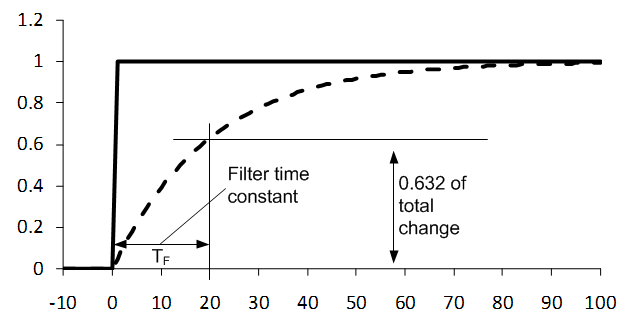
\includegraphics[scale=0.75]{img/lag_Filter.png}
	\caption{Wirkung eines First-Order Lag Filters beim Wechsel des \newline Eingangsignals von 0 auf 1}
	\label{Abb_lag_filter}
\end{figure}

Aus der Abbildung \ref{Abb_lag_filter} wird ersichtlich, wie ein First-Order Lag Filter auf ein starkes Wachstum eines Wertes reagiert. Die durchgezogene Linie, welche beim Zeitpunkt null auf einen Wert von eins steigt, zeigt den Verlauf ohne Filter. Die gestrichelte Linie, welche im Zeitpunkt null beginnt, zeigt den Verlauf mit Filter. T\textsubscript{F} zeigt die Dauer des verwendeten Zeitintervalls. Die schwarzen Linien, beginned bei einem Wert von zwanzig auf der X-Achse, markieren an ihrem Schnittpunkt  mit der gestrichelten Linie den Wert nach der ersten Anwendung des Filters. Dieser Wert liegt bei 63,2\% der eigentlichen Änderung. Bei fortlaufender Zeit nähert sich die gestrichelte Linie der durchgezogen Linie immer weiter an.

\section{Slotted ALOHA Spannungsregler mit Fokus auf Fairness}
Bei den nächsten vorgestellten Methoden wurden Bestandteile des Slotted Aloha Protokolls (Kapitel \ref{capBack:Aloha}) verwendet. Das Slotted Aloha Protokoll arbeitet auf einem geteilten Medium, welches von allen Teilnehmern verwendet wird. Dieses geteilte Medium ist in diesem Fall das in Kapitel \ref{capBack:Stromnetz} vorgestellte Niederspannungsnetz mit den dazugehörigen elektrischen Leitern und dem verbautem Transformator. Die elektrischen Leiter im Niederspannungsnetz bedienen jeweils mehr als einen Anschluss, stehen also mehr als einem Teilnehmer gleichzeitig zur Verfügung. Der Transformator wird ebenfalls von mehr als einem Teilnehmer verwendet. Diese Teilung lässt sich auf seine einzigartige Schlüsselrolle, der Bereitstellung elektrischer Energie, und die Tatsache, dass alle Leiter mit ihm verbunden sind, zurückführen.\\
\begin{figure}[htb]
	\centering
	
\includegraphics[scale=0.75]{img/sharedMedium3.png}
	\caption{Verglich von Aloha Netzwerkprotokoll und Stromnetz}
	\label{Abb_sharedmedium}
\end{figure}
In der Abbildung \ref{Abb_sharedmedium} ist in der oberen Hälfte ein möglicher Aufbau eines Netzes zu sehen, in dem man das Aloha Netzwerkprotokoll, sowohl in der herkömmlichen aber auch in der slotted Variante, verwenden könnte. Die fünf, größeren Kästchen stellen die Teilnehmer dar, die beiden kleineren markieren die Grenzen des Netzes. Die Linien stehen für das eigentliche geteilte Medium. Im unteren Teil des Bildes ist ein möglicher Aufbau eines Niederspannungsnetzes mit einem Transformator und fünf Teilnehmern dargestellt. Das dargestellte Niederspannungsnetz verfügt über nur einen Strahl. Der Transformator wird durch das Kästchen dargestellt, zwei ineinander verschobene Kreise stellen jeweils einen Teilnehmer dar. Die ersichtlichen Ähnlichkeiten der physischen Aufbauten lässt erneut den Schluss zu das sich das geteilte Medium im Fall des Aloha Netzwerkprotokolls und im Fall des Stromnetzes vergleichen lässt.\\
Im Aloha Netzwerkprotokoll werden Informationen mithilfe von Frames transportiert. Im Stromnetz werden elektrische Teilchen über elektrische Leitung transportiert. Ein Frame hat allerdings eine zuvor festgelegte Größe, welche nicht unter- oder überschritten werden darf. Leistung kann über einen beliebigen Zeitraum in jeder technisch machbaren Höhe bezogen werden. Teilt man die Zeit allerdings in diskrete Abschnitte ein, so ergibt sich eine maximale Menge an Leistung, welche in diesem Zeitraum bezogen werden kann. Sollte kein ganzer Zeitslot benötigt werden, gibt es jedoch auch eine Lösung. Im Falle des Aloha Netzwerkprotokolls gibt es die Möglichkeit einen Frame, welcher nicht vollständig mit Daten gefüllt werden kann, mit Fülldaten zu ergänzen, um einen vollständigen Frame zu erhalten. Im Stromnetz wird durch einen niedrigeren Leistungsbezug als eigentlich möglich die Zeit eine Slotes, welcher nicht ganz genutzt werden würde, doch voll ausgenutzt. Im Aloha Netzwerkprotokoll können Kollisionen auftreten. Diese treten immer dann auf, wenn mehr Teilnehmer als erlaubt das geteilte Medium gleichzeitig verwenden. Im Stromnetz gibt es ähnliche Situationen. Die erste wäre, wenn die Spannung bei einem Teilnehmer unter einen Schwellenwert fällt. Bei einem Spannungswert unterhalb dieses Schwellenwertes ist kein weiterer Leistungsbezug aus dem Netz möglich und der Ladevorgang muss an dieser Stelle beendet werden. Die zweite Möglichkeit, wie im Stromnetz eine Kollision auftreten kann, ist wenn der Transformator eine höhere Last ans Netz abgibt als erlaubt. Tritt eine solche Kollision ein sind prinzipiell alle, zu diesem Zeitpunkt Leistung beziehenden, Teilnehmer betroffen. Auch eine solche Kollision führt zu einer Beendigung des aktuellen Ladevorgangs und zur Beendigung des Leistungsbezuges. Der in Kapitel \ref{capBody:VDE} vorgestellte Spannungsregler reagiert nur auf die erste Art der möglichen Kollisionen. Die weiteren Methodiken welche im Folgenden vorgestellt werden reagieren auf eine oder beide Arten der Kollisionen auf verschieden Art und Weisen.
In Kapitel \ref{capBack:Aloha} wurden zwei verschiedene Varianten des Aloha Netzwerkprotokolls vorgestellt, eine herkömmliche und eine slotted Variante. Das Stromnetz gleicht von der Arbeitsweise der Teilnehmer aus gesehen mehr der herkömmlichen Variante. Teilt man allerdings auch im Stromnetz die Zeit in diskrete Schritte ein und erlaubt Änderungen nur zu Beginn eines solchen Schrittes. So entsteht auch im Stromnetz eine Arbeitsweise, welche nun mehr dem Slotted Aloha entspricht. Da nun in dieser Arbeit die Zeit in diskrete, gleich lange Zeitabschnitte eingeteilt wird, wird im Stromnetz die Arbeitsweise des slotted Aloha Netzwerkprotokolls verwendet.

\subsection{Wartezeit über Teilnehmerzahl}
\label{cap:background_sec:SA_participants}
Der in Kapitel \ref{capBody:VDE} vorgestellte Spannungsregler wird um die Behandlung von lokalen Spannungskollisionen, welche bei jedem Teilnehmer individuell passieren können, erweitert. Eine Spannungskollision tritt immer dann auf, wenn der Wert der lokal gemessen Spannung auf unter 88\% der Normspannung fällt. Fällt die Spannung auf einen solch niedrigen Wert kann gemäß dem Spannungsregler keine Leistung mehr aus dem Netz bezogen werden, bis die Spannung wieder auf einen Wert von über 88\% der Normspannung steigt. Ist eine Spannungskollision aufgetreten, wird, geregelt durch den Spannungsregler, der mögliche Leistungsbezug auf null zurückgefahren, der tatsächliche Leistungsbezug wird durch die Filterung der Werte erst langsam auf null reduziert. Im Kollisionsfall wird zudem eine Wartezeit bestimmt. Diese Wartezeit gibt an, wie lange der Teilnehmer nicht mehr versucht Leistung aus dem Netz zu beziehen. Der Wert der Wartezeit wird per Zufall aus einem Intervall heraus bestimmt, unter Verwendung einer gleichverteilten Zufallsfunktion. Das Intervall ist nach unten sowie oben begrenzt. Die untere Grenze ist die Null, was keiner Wartezeit entspricht. Die obere Grenze wird primär durch die aktuelle Anzahl an Teilnehmer bestimmt. Diese Anzahl an Teilnehmern wird über die Anzahl an Nachrichten, welche über das Broadcast System übermittelt wurden, festgestellt. Bleiben Nachrichten komplett aus wird die bisherige Maximalanzahl des aktuellen Tages verwendet. Ein Sonderfall tritt ein, wenn die Menge der Teilnehmer zahlenmäßig höher ist als die Anzahl der Zeiteinheiten zwischen dem aktuellen Zeitpunkt und dem Zeitpunkt an dem das Fahrzeug die Ladestation wieder verlässt. Wenn dieser Fall eintritt, wird das Intervall, aus welchem die Zufallszahl heraus bestimmt wird, nicht von der Anzahl der Teilnehmer nach oben hin begrenzt. Die obere Grenze des Intervalls entspricht dann der Anzahl von Zeiteinheiten zwischen dem aktuellen Zeitpunkt und dem Zeitpunkt an dem das Fahrzeug die Ladestation wieder verlässt.  In mathematischer Schreibweise lässt sich das Intervall wie folgt darstellen [0, max(Teilnehmeranzahl, Zeiteinheiten bis zur Abfahrt)]. Es besteht die Möglichkeit, das wenn die Wartezeit abgelaufen ist wieder oder immer noch eine Spannungskollision vorliegt. Tritt dies ein, wird wieder eine Wartezeit bestimmt. Das Durchlaufen einer Wartezeit bringt keine Garantie am Ende dieser Wartezeit auch wieder einen Ladevorgang aufzunehmen. Diese hier vorgestellte Methodik wurde nur um Funktionalität für Spannungskollisionen erweitert. Wenn eine zu hohe Last vom Transformator abgerufen wird, werden bei dieser Methodik allerdings keine Maßnahmen ergriffen. Diese Methodik wird im weiteren Verlauf der Arbeit mit SA+T bezeichnet.\\
\begin{figure}[htb]
	
\includegraphics[width = \linewidth]{img/SA_participants_Graph2.png}
	\caption{Beispielansicht eins Ladeservice}
	\label{SAPart:Graph}
\end{figure}

In der Abbildung \ref{SAPart:Graph} wird beispielhaft die Situation eines einzelnen Fahrzeuges deutlich, welches an dem aktuellen Zeitpunkt eine Kollision registriert hat und nun eine Wartezeit berechnet. Die angedeutete maximale Wartezeit umfasst für jeden aktiven Teilnehmer, dessen Nachricht über das Broadcast System empfangen wurde eine Zeiteinheit. Die tatsächliche Wartezeit des Teilnehmers lässt sich allerdings nicht im Vorhinein bestimmen, da diese per Zufall aus einem Intervall heraus ermittelt wird.
\begin{table}[htb]
\centering
\begin{tabular}{|l|l|l|}
\hline
Zeitpunkt & Fahrzeug Nr. & Ladestand (in \%) \\ \hline \hline
10:00     & 1            & 12,6      \\ \hline
11:30     & 2            & 55,3      \\ \hline
          & 3            & 66,8      \\ \hline
15:00     & 1            & 40,7      \\ \hline
          & 2            & 84,1      \\ \hline
          & 3            & 94,2      \\ \hline
\end{tabular}
\caption{Situation von drei verschiedenen Fahrzeugen zu verschiedenen Zeitpunkten}
\label{tab:example1}
\end{table}

In der Tabelle \ref{tab:example1} ist exemplarisch die Situation von drei Fahrzeugen aufgezeigt, welche zu unterschiedlichen Zeiten ankommen und bei der Ankunft über verschiedene Ladestände verfügen. Die Fahrzeuge werden anhand ihrer Nummer in der mittleren Spalte identifiziert. Alle drei Fahrzeuge beginnen den jeweiligen Ladeservice und beginnen so auch Ladevorgänge. In diesem Beispiel tritt um 15:00 am Nachmittag bei allen drei Ladevorgängen eine Kollision auf. Da die Kollision bei allen Teilnehmern auftritt berechnen auch alle Teilnehmer eine Wartezeit. Das Intervall, aus dem diese Wartezeit bestimmt wird, ist für alle Teilnehmer gleich, es lautet [0,3]. Welche Wartezeiten die Teilnehmer tatsächliche abwarten müssen entscheidet allerdings das Ergebnis der Zufallsfunktion.

\subsection{Wartezeit über Teilnehmer und Fahrzeugparameter}
\label{cap:background_sec:SA_waitingTime}
Ähnlich zu dem Vorgehen in Kapitel \ref{cap:background_sec:SA_participants}, bei der Methodik SA+T, wird auch bei diesem Ansatz der in Kapitel \ref{capBody:VDE} vorgestellte Spannungsregler erweitert. Auch bei diesem Ansatz werden lediglich Spannungskollisionen betrachtet und es werden keine aktiven Maßnahmen bei einer zu hohen Last am Transformator ergriffen. Diese Methodik wird im Folgenden mit SA+T+F bezeichnet. Der Unterschied zur Methodik SA+T ist die Art und Weise der Berechnung der Wartezeit. Der Wert der Wartezeit wird auch hier per Zufall aus einem Intervall heraus bestimmt. Der Unterschied liegt in der Art der Bestimmung der oberen Grenze dieses Intervalls. Die obere Grenze wird durch Ausführung einer Formel bestimmt, welche von drei Parametern abhängt.  Der erste Parameter gibt an wie viele Zeiteinheiten, zwischen dem aktuellen Zeitpunkt und dem Zeitpunkt, an dem das Fahrzeug die Ladestation wieder verlässt, liegen. Dieser Parameter wird im Folgenden mit „verbleibender Zeit“ oder t\textsubscript{V} bezeichnet. Der zweite Parameter gibt an, wie viel Zeit noch benötigt wird, um den Akku des Fahrzeuges auf einen Ladestand von 100\% zu bringen. Für diese Berechnung wird allerdings die Normspannung verwendet und nicht die aktuell gemessene Spannung. Dieser Parameter wird im Folgenden mit „verbleibender Ladezeit“ oder t\textsubscript{L} bezeichnet. Die beiden Parameter, verbleibende Zeit und verbleibende Ladezeit, werden lokal von jedem Teilnehmer für sich selbst bestimmt, sie benötigen dafür keinen weiteren Input. Der dritte Parameter ist die aktuelle Anzahl an Teilnehmenden T. Diese Parameter wurden gewählt mit dem Ziel Fahrzeuge, welche erst weniger geladen habe, oder Fahrzeuge, deren Abfahrt kurz bevorsteht, besserzustellen. Durch den Einfluss der Teilnehmerzahl, wird aber auch die Aktivität im Netz mit in Betracht gezogen. Diese drei Parameter, die verbleibende Zeit t\textsubscript{V}, die verbleibende Ladezeit t\textsubscript{L} und die Anzahl der Teilnehmer T werden in folgende Formel eingesetzt um die obere Grenze G\textsubscript{O}:
\begin{align}
	G\textsubscript{O} = \frac{t\textsubscript{V} - t\textsubscript{L}}{T}
	\label{SA:formel4}
\end{align}
Der Ergebnisbereich der Formel \ref{SA:formel4} ist nach oben durch den Faktor 't\textsubscript{V} - t\textsubscript{L}' begrenzt und nach unten aufgrund der Division des Faktors durch minus unendlich. Das Ergebnis dieser Formel beschränkt nun das Intervall, aus dem die Wartezeit bestimmt wird, nach oben.  Die Subtraktion von der verbleibenden Ladezeit und der verbleibenden Zeit, gibt nun an, wie viel Zeit das Fahrzeug neben der, welche zum Laden benötigt wird, noch zusätzlich hat. Diese Zeit würde das Fahrzeug also nicht zum Laden benötigen. Ein Sonderfall tritt auf, wenn das Ergebnis dieser Formel kleiner ist als eins. Dies kann passieren, wenn etwa die verbleibende Zeit geringer ist als die verbleibende Ladezeit. Tritt dieser Fall ein wird erneut eine obere Grenze für das Intervall bestimmt. Dies ist notwendig, da das Ergebnis der Formel \ref{SA-formel5} die obere Grenze eines Intervalls berechnet, aus welchen eine ganze Zahl gezogen werden soll. Ist die obere Grenze nun aber kleiner als eins und die untere Grenze ist null, so gibt es nur eine ganze Zahl in diesem Intervall und die Verwendung der Zufallsfunktion würde keinen Mehrwert bringen. Tritt aber dieser Fall ein muss eine andere Formel verwendet werden. Die Formel, die in diesem Fall verwendet wird, hat nur einen Parameter. Dieser Parameter ist die zuvor berechnete obere Grenze des Intervalls, bezeichnet mit G\textsubscript{alt}. Zur Bestimmung des neuen Wertes wird folgende Formel verwendet \\
\begin{align}
	G\textsubscript{O} = 10 \cdot (1 - e^{G\textsubscript{alt} - 1}) + 1
	\label{SA-formel5}
\end{align}
Der Parameter der Formel \ref{SA-formel5} liegt im Bereich von minus unendlich bis eins. Die Formel wurde entwickelt mit dem Ziel Werte zwischen eins und elf zu liefern, wobei sich eine anfängliche Differenzierung der Ergebnisse bei kleiner werdenden Werten des Parameters einstellen sollte. Das Ergebnis dieser Formel grenzt nun das Intervall, aus dem die Wartezeit bestimmt wird, nach oben ab. Das Verhalten während einer Wartezeit, welche mithilfe dieser Formel \ref{SA-formel5} abgegrenzt wurde, kann sich von dem Verhalten einer Wartezeit welche durch Formel \ref{SA:formel4} abgegrenzt wird unterscheiden. Wenn eine solche Wartezeit das erste Mal bestimmt wird, unterscheidet sich das Verhalten in drei Punkten. Der Erste wäre, dass die Verbindung zum Netz nicht getrennt wird, es wird also weiterhin Leistung aus dem Netz bezogen. Der zweite Unterschied liegt in der Bestimmung der möglichen Ladeleistung, statt mit der Formel \ref{Main_formula3} wird, entgegen dem eigentlich verwendetem Spannungsregler, die Formel \ref{Main_formula1} verwendet. Der dritte Unterschied ist das veränderte Verhalten beim Auftreten von Kollisionen, diese werden nicht beachtet und es wird nicht auf sie reagiert. Eine solche Art der Wartezeit kann allerdings nicht mehrmals direkt hintereinander wahrgenommen werden. Tritt nach Beendigung dieser Wartezeit sofort wieder eine Kollision auf, muss eine normale Wartezeit abgewartet werden, auch wenn das Intervall mithilfe der Formel \ref{SA-formel5} begrenzt wurde. Nach dieser Wartezeit ist eine solche Sonderbehandlung allerdings wieder möglich.\\
\begin{figure}[htb]
	
\includegraphics[width = \linewidth]{img/SA_waiting_Graph4.png}
	\caption{Beispielansicht eines Ladeservices}
	\label{SAWait:Graph}
\end{figure}

In der Abbildung \ref{SAWait:Graph} ist eine exemplarische Darstellung einer Situation eines Fahrzeuges deutlich, welche zu diesem aktuellen  Zeitpunkt eine Kollision registriert. Oberhalb sind die beiden Parameter „verbleibende Zeit“ und „verbleibende Ladezeit“ angetragen. Unterhalb verdeutlicht eine gestrichelte Linie das Ergebnis der Subtraktion dieser beiden Werte. Die vertikalen Linien stehen für die Aufteilung nach der Division durch die Anzahl der Teilnehmer. Ebenfalls angezeigt wird die Länge eines dann verblieben Teiles des Ergebnisses der Subtraktion, die Anzahl der Zeiteinheiten eines solchen Restes begrenzt in diesem Fall das Intervall der Wartezeit noch oben.\\
\begin{table}[htb]
\centering
\begin{tabular}{|l|l|l|l|}
\hline
Zeitpunkt & Fahrzeug Nr. & Ladestand & Abfahrtszeitpunkt \\ \hline \hline
10:00     & 1            & 12,6      & 19:00             \\ \hline
11:30     & 2            & 55,3      & 19:00             \\ \hline
          & 3            & 66,8      & 19:00             \\ \hline
15:00     & 1            & 40,7      & 19:00             \\ \hline
          & 2            & 84,1      & 19:00             \\ \hline
          & 3            & 94,2      & 19:00             \\ \hline
\end{tabular}
\caption{Situation von drei verschiedenen Fahrzeugen zu verschiedenen Zeitpunkten}
\label{tab:example2}
\end{table}

In der Tabelle \ref{tab:example2} wird das Beispiel aus Tabelle \ref{tab:example1} aus Kapitel \ref{cap:background_sec:SA_participants} wiederaufgegriffen. Berechnet man nun allerdings die Wartezeit mit der hier vorgestellten Methodik weichen die Ergebnisse voneinander ab. Für das Fahrzeug mit der Nummer 1 wurde bei einer verbleibenden Zeit von vier Stunden und 40,7\% Ladestand eine maximale Wartezeit von 60 Zeiteinheiten bestimmt. Beim Fahrzeug 2 sollte nun bei selber verbleibender Zeitmenge aber höherem Ladestand auch eine höhere, maximale Wartezeit berechnet werden. Die maximale Wartezeit für das Fahrzeug 2 beträgt 75 Zeiteinheiten, somit tritt ein, was gemäß der abgeänderten Berechnung eintretten soll, die maximale Wartezeit von Fahrzeug 2 ist höher als die von Fahrzeug 1. Die Situation zwischen Fahrzeug 3 und Fahrzeug 2 ist ähnlich zu der zwischen Fahrzeug 1 und 2. Fahrzeug 3 sollte eine höhere maximale Wartezeit aufweisen als Fahrzeug 2 und bei 78 Zeiteinheiten ist dies auch der Fall.  

\section{Slotted ALOHA Spannungsregler mit Transformatorlaststeuerung}
Die Laststeuerung am Transformator soll dazu beitragen die Ausgangsleistung des Transformators im Niederspannungsnetz besser zu regeln und zu limitieren. Die Limitierung der Ausgangsleistung trägt erstens zur Schonung des Transformators an sich bei, aber auch die sich im Stromnetz bewegende Leistung wird limitiert. Die Regelung der möglichen Transformatorlast erfolgt gemäß dem Vorbild des VDE Spannungsregler, bekannt aus dem Kapitel \ref{capBody:VDE}. Die mögliche Ladeleistung wird abhängig von der aktuellen Transformatorlast geregelt. Es wurde ein Limit festgelegt, welches als Obergrenze verwendet wird. In einem Bereich von 80\% bis 100\% wird die mögliche Ladeleistung linear reduziert. Bei einer Transformatorlast von weniger als 80\% steht die mögliche Ladeleistung komplett zur Verfügung. Bei einer Transformatorlast, welche über dem Limit liegt, kann keine Ladeleistung mehr abgerufen werden.  \\
\begin{figure}[htb]
	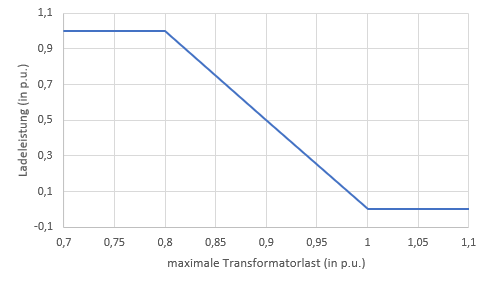
\includegraphics[width = \linewidth]{img/TrafoGraph1.png}
	\caption{Transformatorlast zu Leistungsverhältnis}
	\label{SATrafo:Graph}
\end{figure}

In der Abbildung \ref{SATrafo:Graph} zeigt die mögliche Ladeleistung bei dem prozentualen Anteil der maximalen Transformatorlast. Auf der Y-Achse ist die mögliche Ladeleistung angetragen, wobei die eins für die höchstmögliche Leistung steht und null dafür, das keine Leistung abrufbar ist. An der X-Achse werden die aktuell anliegenden Prozent der Normspannung angetragen. An dem Graphen ist ersichtlich wie sich eine ansteigende Transformatorlast auf die mögliche Ladeleistung auswirkt. Ebenso wird im Vergleich mit der Abbildung \ref{Abb_VDEController} ersichtlich, wie die Arbeitsweise der beiden Regler übereinstimmt. Der Faktor gibt an welcher Anteil der Ladeleistung bei der aktuellen Transformatorlast verfügbar ist. Ergebnisse größer als eins werden auf eins reduziert, da alle Werte größer als eins in einer höheren Ladeleistung als möglich resultieren würden. Der Wert des Faktors F\textsubscript{T} wird mit folgender Formel bestimmt \\
\begin{center}
	$ F = \begin{cases}
	1 &  \text{$<$ 80\% maximaler Last} \\
	0 &  \text{$>$100\% maximaler Last} \\
	- \frac{10}{403333} \cdot L\textsubscript{T} + 5 & \text{$>$ 80\%, $<$ 100\% maximaler Last}
	\end{cases}$
\end{center}
Der Wert der aktuellen Transformatorauslastung wird ähnlich zu der Anzahl der Teilnehmer über das Broadcastsystem verteilt. Liegt der Wert nicht vor, wird ein Wert nahe am Limit gewählt, um die Last so niedrig wie möglich zu halten, aber dennoch noch eine Lastbezug zu zulassen. Der Faktor der Transformatorlast wird ebenso wie der Faktor zur Spannung in der Formel \ref{Main_formula1} berücksichtigt, dadurch verändert sich die Formel \ref{Main_formula3} wie folgt
\begin{align}
	P\textsubscript{L} = U\textsubscript{A} \cdot I\textsubscript{F} \cdot F\textsubscript{S} \cdot F\textsubscript{T} \label{Main_formula4}
\end{align}
Neben der Formel zur Berechnung der möglichen Leistung, wird auch der verwendete Lag-Filter rekonfiguriert. Am Vorgehen bei der Erhöhung der Werte wird nichts verändert, lediglich das Verhalten be der Verringerung von Werten wird angepasst. Die Gründe für eine Verringerung der Leistung sind eine gesunkene Stromstärke, eine gesunkene Spannung oder ein verändertes Ergebnis der beiden Faktoren für Spannung und Transformatorlast. Das geänderte Verhalten tritt nur auf, wenn eine Transformatorkollision vorliegt, da eine Kollision einen laufenden Ladevorgang beendet, fällt nach einer Kollision immer der Wert der bezogenen Leistung. Tritt eine Transformatorkollision auf, ergibt die Formel \ref{Main_formula4} immer 0. der In Kapitel \ref{capBody:VDE} eingeführte Filter würde 63,2 \% der nötigen Änderung vornehmen, der hier vorgestellte Filter nimmt jedoch nur 36,8 \% der Änderung vor.

%\chapter{How To in Deutsch}
\label{sec:howtodeutsch}

For english version, see below.

Hier kann beschrieben werden, wie man das Problem gelöst hat und alle Schritte auf dem Weg zum Ergebnis.

\section{How To: Wie man eine Abschlussarbeit schreibt}
In diesem Abschnitt werden einige hilfreiche Tipps und Tricks für das Schreiben und im Umgang mit Latex vorgestellt.
Für Überschriften kann man einheitliches ``Titlecase'' verwenden.

\section{Latex-Umgebung}
Fast jeder Texteditor eignet sich dazu, um Latex zu schreiben. Empfehlenswert ist aber eine Entwicklungsumgebung wie z.B. TeXStudio.

\section{Beispiel für eine Abbildung}
\begin{figure}[h!]
	\begin{center}
		
\includegraphics[width=7cm]{img/logochair.pdf}
		\caption{Beispiel für eine Beschriftung.}
		\label{fig:ToUseWithReference}
	\end{center}
\end{figure}

Durch die \texttt{\bslash label} kann auf die Bilder mit
\texttt{\bslash ref} verwiesen werden. Es ist wichtig, im Text kurz die Abbildung zu beschreiben. Zum Beispiel: In Abbildung~\ref{fig:ToUseWithReference} sieht man das Logo des Lehrstuhls, das als Beispiel einer Abbildung dienen soll. In blau ist der Text dargestellt, in schwarz das Symbol des Lehrstuhls.

Die Tilde sorgt dafür, dass kein Umbruch zwischen Abbildung und Zahl vorkommt.


\section{Beispiel für eine Tabelle}
Klar strukturierte Tabellen lassen sich mit dem Booktabs-Paket erstellen, wie man in Tabelle~\ref{table:ranking} sehen kann.

\begin{table}
	\begin{center}
		\begin{tabular}{cl}
			\toprule
			\textbf{Ranking} & \textbf{Letter} \\
			\midrule
			1 	& A \\
			2 	& B\\
			3	& C\\
			4	& D\\
			5	& E\\
			6	& F\\
			7	& G\\
			\bottomrule
		\end{tabular}
		\caption{Ranking der Buchstaben im Alphabet.}
		\label{table:ranking}
	\end{center}
\end{table}




\section{Beispiele für Referenzen}
Die Literaturhinweise werden im Text z.B.\ folgendermaßen verwendet:\\
``..., wie in \cite{architecturemobilep2p} gezeigt.'' Der Stil der Referenz kann in der Datei ``ThesisCNaCC.tex'' angepasst werden (z.b. nur Zahlen anzeigen). Bei den meisten Papern kann direkt eine Bibtex-Quelle heruntergeladen werden (z.B. auf Google Scholar, Springer etc.). Zur Verwaltung der Literatur bieten sich Programme wie Jabref, Mendeley etc. an.

\section{Schrifttypen}
Als Schrifttyp wird Arial oder Roman empfohlen. Bitte beachten, dass
Größen und Einheiten eine eigene Schreibweise haben:
\begin{description}
	\item[Kursivschrift:] physikalische Größen (z.B.~$U$ für Spannung),
	Variablen~(z.B.~$x$), sowie Funktions- und Operatorzeichen, deren
	Bedeutung frei gewählt werden kann (z.B.~$f(x)$)
	\item[Matheformeln im Mathemodus:] $\frac{1}{1} \cdot 3 = 3$
\end{description} 

\section{Code der Arbeit}
\subsection{GitLab} Am Lehrstuhl gibt es ein GitLab. Hier könnt ihr euren Code mit Versionskontrolle verwalten,
und am Ende kann euer Betreuer ebenfalls auf den Code zugreifen. 

Kontaktiert bei Interesse euren Betreuer, dieser wird euch weitere Details geben!

\subsection{Hardware}
Falls ihr mehr Rechenpower für euren Code/Simulationen benötigt, wendet euch bitte an euren Betreuer!


\subsection{Code einfügen} Bitte kopiert nicht euren gesamten Code in die Arbeit! An manchen Stellen kann es aber sinnvoll sein,
kurze Abschnitte zu zeigen. Das geht am besten mit Listings, as shown in Listing~\ref{helloJava}:

\begin{lstlisting}[language=java, caption=Hello World in Java, label=helloJava]
public static void main (String[]args) {
System.print.out("Hello World");
}
\end{lstlisting}

Man kann den Code auch direkt aus einer Datei darstellen (Datei ist nicht vorhanden, daher auskommentiert).
%\lstinputlisting[language=Python, caption=Direkt aus Datei, label=direktDatei]{source_filename.py}

Falls die Darstellung noch nicht gefällt, kann es angepasst werden: \url{https://en.wikibooks.org/wiki/LaTeX/Source_Code_Listings#Settings}

\section{Abkürzungen}
Falls man viele fachspezifische Abkürzungen in der Arbeit verwendet, bieten sich Latex-Pakete zur Unterstützung an, zum Beispiel acronym oder glossary.
Beispiel acronym-Paket: Eine \ac{VM} wird benutzt. Mehrere \acp{VM} sind besser als eine \ac{VM}.
Das ist eine lange Abkürzung: \ac{ssla}, bei der der Plural anders ist: \acp{ssla}.



\chapter{How To in English}
Here, you can describe how the problem was solved and the steps taken to obtain the results.

\section{Latex-Environment}
Almost every text editor can be used to write latex. However, an IDE is recommended e.g TeXStudio.


\section{How To: Write a Thesis}
In this section, some useful tricks for writing and for using latex are presented.
For headings in general, you can use ``Titlecase'' for a consistent appearance.

\section{Example for a Figure}
	\begin{figure}[h!]
		\begin{center}
			
\includegraphics[width=7cm]{img/logochair.pdf}
			\caption{Example for a title of a figure.}
			\label{fig:ToUseWithReference}
		\end{center}
	\end{figure}
	
	With the help of \texttt{\bslash label}, figures and tables can be addressed with the command \texttt{\bslash ref} 
	It is important, to describe the figure in the text. For example: In Fig.~\ref{fig:ToUseWithReference}, one can see the logo of the chair. The text is shown in blue, and the in black the symbol of the chair.
	
	The tilde prevents a linebreak between Figure and the number.
	
	\section{Example for a table}
	Clearly structured tables can be realized with the packet booktabs as you can see in Table~\ref{table:ranking}.
	
	\begin{table}
		\begin{center}
			\begin{tabular}{cl}
				\toprule
				\textbf{Ranking} & \textbf{Letter} \\
				\midrule
				1 	& A \\
				2 	& B\\
				3	& C\\
				4	& D\\
				5	& E\\
				6	& F\\
				7	& G\\
				\bottomrule
			\end{tabular}
			\caption{Ranking of letters in the alphabet.}
			\label{table:ranking}
		\end{center}
	\end{table}
	
	
	\section{Example for References}
	The literature reference in the text are used as follows:\\
	``..., as shown in \cite{architecturemobilep2p}.'' The Style of the reference can be adapted in the file ``ThesisCNaCC.tex'' (e.g. show only numbers). For the most papers, you can directly download the Bibtex source (e.g. at Google Scholar, Springer etc.). For an easier management, you can use programs like Jabref, Mendeley etc.
	
	\section{Fonts}
	As font, Arial or Roman is recommended. Please note that some units have their own font:
	\begin{description}
		\item[Italic:] physical units(e.g.~$V$ for Voltage),
		Variables~(e.G.~$x$), and functions and operators (e.G.~$f(x)$)
		\item[Mathematical formulas in math mode:] $\frac{1}{1} \cdot 3 = 4$
	\end{description} 
	
	\section{Code of the Thesis}
	\subsection{GitLab} At the chair, there is a GitLab you can use for managing your code with version control. In the end, your supervisor can easily access this code.
	
	If interested, please contact your supervisor!
	
	\subsection{Computing Power}
	If you need hardware for your code/simulations, please contact your supervisor!
	
	
	\subsection{Insert Code } Please do not copy your complete code in the thesis! But on some points it can be helpful to show snippets. You can use Listings:
	
	\begin{lstlisting}[language=java, caption=Hello World in Java, label=helloJava]
	public static void main (String[]args) {
	System.print.out("Hello World");
	}
	\end{lstlisting}
	
	You can import the code directly from a file, too (File does not exist here)
	%\lstinputlisting[language=Python, caption=Direkt aus Datei, label=direktDatei]{source_filename.py}
	
	The appearance can be adapted: \url{https://en.wikibooks.org/wiki/LaTeX/Source_Code_Listings#Settings}
	
	\section{Abbreviations}
	If you are using many abbreviations, you can use latex-packages like acronym or glossary. For exmaple a \ac{VM} is used. More \acp{VM} are better than one \ac{VM}.
	This is a very long abbreviation in german: \ac{ssla}, with a different plural: \acp{ssla}.
	


%\chapter{Ergebnisse/Results}
Hier werden die Ergebnisse gezeigt und beschrieben. Vergesst nicht eine ordentliche Beschriftung zu erstellen!

--------
\newline
Here, results are shown and described. Do not forget proper labels for figures!

%\chapter{Related Work}
\section{Konzepte mit Quality of Service Ansatz}
Anders als die bisher vorgestellten Konzepte, welche zwar ein ähnliches oder das selbe Ziel haben, wie diese Arbeit, deren eingeschlagenWeg sich allerdings grundlegenden unterscheidet, gibt es auch Ansätze, welche sich Ideen und Konzepten der Netzwerktechnik bedienen und diese auf das Stromnetz anwenden. \\
In Ihrer Arbeit \cite{RW_3_1} legen  Ammar  Alyousef und Hermann de Meer ein Konzept dar, für einen Kontrollmechanismus, welcher dezentral an den Anschlüssen der jeweiligen Ladegeräte ansetzt. Der Kontrollmechanismus überprüft die Einhaltung der Grenzwerte für die Last am Transformator sowie der Spannung an den einzelnen Anschlüssen. Die Zustände der gemessen Werte werden anhand eines Ampelschemas eingeteilt, wobei grün keinen Anlass zu Veränderungen Anzeigt, gelb eine leichte Änderung und rot eine drastische Änderung, um die Werte innerhalb der jeweils zulässigen Bereiche zuhalten. Sollten die Werte nun einen Anlass vermitteln, welcher eine Änderung notwendig macht, verwendet man hier das Prinzip des TCP-Slow Starts, welches aus der Netzwerktechnik stammt. Der Aufbau des verwendeten Netzes sowie die bereits anliegenden Lasten, ohne die Ladegeräte, wurden aus der Realität übernommen. Es werden insgesamt vier verschiedene Szenarien getestet, kein Ladegerät am Netz, alle Ladegeräte unter Vollast am Netz, sowie zwei verschiedene Smart Charging Ansätze, einmal der in der Arbeit selbst vorgestellte und ein Ansatz, der einen endlichen Automaten verwendet und aus vorhandener Literatur herausgenommen wurde, als Vergleichsinstanz. Das Ergebnis zeigt, das sich die Verwendung der beiden Smart Charging Ansätze, vor allem in der Qualität der zur Verfügung stehenden Elektrizität auszahlt, aber auch bei der Menge der transportierten Energie. Jedoch stellt sich dar das der Smart Charging Ansatz, welcher den TCP-Slow Start verwendet, fairer ist bei der Verteilung zwischen den Ladestationen. Die Anordnung der Ladestationen unterscheidet sich allerdings dahingehend von der Verteilung in dieser Arbeit, da hier davon ausgegangen wird, das sich die Ladestationen stärker im Netz verteilen, da mehr von Ihnen angeschlossen wurden. Auch in der hier vorgestellten Arbeit unterscheiden sich die verwenden Parameter von denen in dieser Arbeit verwendeten. In der hier vorgestellten Arbeit orientriert man sich lediglich an den Auslastungsdaten des Stromnetzes, während in dieser Arbeit auch Daten des jeweiligen Elektrofahrzeugs berücksichtigt werden, wie Ladezustand des Akkus, sowie der nächste Abfahrtszeitpunkt.
\section{Konzepte zur Verbesserung der Netzauslastung}
Die Bemühungen das bestehende Stromnetz auf die Zukunft vorzubereiten und dafür mehr Inteligenz in das Netz zu integrieren sind nicht nur auf die in dieser Arbeit beschränkt. \\
S. Sangob und S. Sirisumrannukul \citet{RW_1_1} haben in Ihrer Arbeit ebenfalls das Ziel das Spannungslevel auch bei mehreren Ladevorgängen stabil zu halten, und so das Netz bestmöglich zu nutzen. Dieses Ziel versuchen sie über eine Partikelschwarmoptimierung zu erreichen, welche auf allen drei Phasen eins 120V Netzes agiert. Das Ergebnis dieser Optimierung ist eine etwa 15\% höhere Leistungsabgabe des Transformator, welche durch eine Erhöhung des Spannungsniveaus bei gleichbleibender Stromstärke erreicht wurde. Die von Ihnen angestrebte Optimierung greift  am Transformator des Niederspannungsnetzes, sowie den mit dem Transformator verbunden Kondensatoren an, also an anderer Stelle, als die in dieser Arbeit thematisierte Lösung, welche am Hausanschluss bzw. erst am Ladegerät selbst ansetzt. Dieser Unterschied beeinflusst auch, an welchem Punkt des Netzes die Spannungswerte gemessen werden, welche von Ihnen nur am Transformator erfasst werden, während die Werte in dieser Arbeit an allen Anschlusspunkten berücksichtigt werden, was die Übertragungsverluste und die Netztopologie mehr berücksichtigt. Ebenso unterscheiden sich die Zielen zwischen der hier genannten Arbeit und dieser Arbeit, während in der hier genannten Arbeit das Ziel war die Qualität der übertragen Spannung zu erhöhen, ist das Ziel dieser Arbeit die Quality of Service des Ladevorgangs von Elektrofahrzeugen, abhängig von Ladezustand des verbauten Akkus und der für den Ladevorgang verfügbaren Zeit, zu erhöhen.
\\
Einen andern Ansatz verfolgen M. Nour et al. in Ihrer Arbeit \cite{RW_2_1}. In Ihrer Arbeit stellen Sie einen Ansatz vor, indem Stromanbieter einen Zweipreistarif anbieten, ein höherer Preis für Zeiten mit höherer Last und ein zweiter, niedrigerer preis, bei geringerer Last, bestimmt wird diese Auslastung am Transformator des Stromnetzes. Dieses Tarifsystem macht das laden außerhalb von Lastzeiten wirtschaftlich attraktiver, was dazu führen soll, das Halter von Elektrofahrzeugen diese Zeiten zum Laden nutzen und eben nicht die Zeiten, wo auch ohne Ladevorgänge schon eine hohe Last auf dem Netz liegt. Diese Zeitsteuerung wird in einen Fuzzy-Controller integriert, welcher neben dem Preis auch den Ladezustand des Fahrzeugs berücksichtigt und so die mögliche Ladeleistung des Fahrzeuges bestimmt. Jedoch steht anders als in dieser Arbeit nicht der Quality of Service Aspekt, einer möglichst zeitnahen,  dem nächsten Abfahrtszeitpunkt entsprechende Ladung im Vordergrund, sonder eher der wirtschaftliche Aspekt, mit der Verwendung von möglichst günstig zur Verfügung stehender Elektrizität. Durch die unterschiedliche Ziele der Arbeiten werden auch unterschiedliche Daten herangezogen, in der hier vorgestellten Arbeit wird nur der Ladezustand des verbauten Akkus betrachtet, während in dieser Arbeit auch die Zeit welche das Fahrzeug am Ladegerät verbracht hat bzw. noch verbringen wird. Des weiteren kontrolliert die hier vorgestellte Arbeit die Auslastung des Netzes nur passiv, da die Preise nur fallen, wenn die Auslastung niedrig ist und so die Belastung durch die Ladevorgänge verkraftbar ist.\\




%-kommunukationprotokolle im EV charging
%fair queueing aus 2013 nimmt auch protokolle
%klimaanlage  in mim/max aufteilung

%tcp slowstart mit ev (amar)

%\chapter{Zusammenfassung}

Am Schluss werden noch einmal alle wesentlichen Ergebnisse
zusammengefasst.  Hier können auch gemachte Erfahrungen beschrieben
werden.  Am Ende der Zusammenfassung folgt ein Ausblick,
der die zukünftige Entwicklung der behandelten Thematik aus der Sicht
des Autors darstellt.


--------------
\newline
In the end, all relevant results are summarized. All experiences can
described. At the end, future work is described. i.e. the future research questions
and the development of the problem.

%
\chapter{Zusammenfassung Neu} 
The problem of a voltage drop in a low voltage network, after the connected peers drew a too high load, motivates an investigation. The power grid scenario with too many users using the grid, for example, to charge electric cars, can be seen as a multiple access problem known from computer networking. An example of a multiple access protocol
 would be the ALOHA protocol. The aloha protocol was invented in 1970 for coordinating and arbitrating access to a shared communication network, this means it falls into the class of multiple access protocols. There are two forms of the ALOHA protocol, that will be looked at here, pure and slotted ALOHA. Through the usage of this protocol, the aim is to improve the handling of high loads on a low voltage sub-network, which can be created by charging multiple electric cars at once. \\
The evaluation of the methods mentioned beforehand will be done using the co-simulation framework mosaik, which couples a power flow solver(PyPower) and our implementation of the ALOHA algorithm. This co-simulator needs predefined networks for a functioning operation, the ones used here are a low voltage grid from a small town in Bavaria and the IEEE906, to representative European network. The results received after the simulation will show if the ALOHA protocol helps by handling these high loads. The voltage levels over time, the delivered power and the overall usage factor of the network will reveal the differences that can be achieved, when using the ALOHA protocol, both in the pure and in the slotted version, over the charge as you come principle.\\
Another set of results can be received when altering the networks and/or the settings attached to it. A first thing could be modifying the voltage boundary at certain places inside the subnetwork, to avoid a too narrow gap between the start value, without an actual load on the subnetwork, and the lower border, which makes devices cut down on power usage. Another possibility is, to alter the network itself, by adding additional paths to the network, so that a radial network turns into a meshed network, where there can be more than one way from the source to a destination.



%\appendix
%\chapter{Abkürzungsverzeichnis}
\begin{acronym}
	\acro{VM}{Virtual Machine}
	\acro{CD}{Compact Disc}
	\acro{ssla}{sehr sehr lange Abkürzung}
	\acroplural{ssla}[ssla'en]{sehr sehr lange Abkürzungen}
\end{acronym}
%\chapter{Ein Beispiel für einen Anhang}

Beispiel für eine Tabelle:

\begin{table}[htbp]
  \begin{center}
    \begin{tabular}{lcr}
      \hline
      left & center & right\\
      \hline
      entry & entry & entry \\
      entry & entry & entry \\
      entry & entry & entry \\
      \hline
    \end{tabular}
    \caption{Beispiel für eine Beschriftung.}
    \label{tab:ToRef}
  \end{center}
\end{table}

%\listoffigures
%\listoftables

% References (Literaturverzeichnis):
% a) Style alpha, (with numbers: use unsrt):
\bibliographystyle{alpha}
% b) The File:
\bibliography{Bibliography}


%%%%%%%%%%%%%%%%%%%%%%%%%%%%%%%%%%%%%%%%%%%%%%%%%%%%%%%%%%%%


%%%%%%%%%%%%%%%%%%%%%%%%%%%%%%%%%%%%%%%%%%%%%%%%%%%%%%%%%%%%


%%%%%%%%%%%%%%%%%%%%%%%%%%%%%%%%%%%%%%%%%%%%%%%%%%%%%%%%%%%%
\end{document}
zz